%%%%%%%%%%%%%%%%%%%%%%%%%%%%%%%%%%%%%%%%%%%%%%%%%%%%%%%%%%%%%%%%%%%%%%%%%%%%%%%
%% 2.- DESARROLLO DEL PROYECTO
%%%%%%%%%%%%%%%%%%%%%%%%%%%%%%%%%%%%%%%%%%%%%%%%%%%%%%%%%%%%%%%%%%%%%%%%%%%%%%%

\cleardoublepage
\chapter{Desarrollo del proyecto}
\chaptermark{Desarrollo del proyecto}

\label{chap:desarrolloProyecto} % etiqueta para poder referenciar luego en el texto con ~\ref{sec:intro}
% \addcontentsline{toc}{chapter}{Introducción, Objetivos, Metodología y Planificación

En las siguientes secciones se detalla de forma estructurada el desarrollo de cada una de las partes que componen este proyecto.


\section{Programación iPro}
\label{sec:programacionipro}
Como ya se ha explicado en los capítulos anteriores, el destino del iPro es la programación de la UTA existente en el supermercado. En el \hyperref[chap:anexoUTA]{Anexo~\ref{chap:anexoUTA}} se describe detalladamente qué es una UTA y todos los elementos de los que se puede componer. Para el caso que nos atañe, la \hyperref[tab:especificacionesUTA]{Tabla~\ref{tab:especificacionesUTA}} recoge las especificaciones concretas del control.

\begin{table}[H]
    %\centering
    \begin{center}
      \setlength\arrayrulewidth{2pt}
      \resizebox{0.8\linewidth}{!}{\begin{tabular}{ | c | c c c c | }
        %\Cline{2pt}{2-5}
        \hhline{|*{5}{-}}
        \cellcolor{lightgray}\textbf{GRUPO} & \multicolumn{1}{c|}{\cellcolor{lightgray}\textbf{Entrada analógica}} & \multicolumn{1}{c|}{\cellcolor{lightgray}\textbf{Salida analógica}} & \multicolumn{1}{c|}{\cellcolor{lightgray}\textbf{Entrada digital}} & \cellcolor{lightgray}\textbf{Salida digital}   \\ \hline
        \footnotesize{\textbf{Ventiladores}} &  & \parbox[c][1.6cm]{0.2\linewidth}{\centering\footnotesize{Ventilador impulsión\\Ventilador retorno}}  & \parbox[c][2.6cm]{0.2\linewidth}{\centering\footnotesize{Seguridad Ventilador impulsión\\Seguridad Ventilador retorno}} &  \\ \hline
        \footnotesize{\textbf{Filtros}} & & & \footnotesize{\parbox[c][2cm]{0.2\linewidth}{\centering{Filtro entrada\\Filtro salida\\Filtro retorno}}} & \\ \hline
        \footnotesize{\textbf{Humectador}} & \footnotesize{\parbox[c][1.2cm]{0.2\linewidth}{\centering{Humedad de retorno\\Humedad exterior}}} & & \centering\footnotesize{Indicador nivel agua} & \footnotesize{ON/OFF Humectador} \\ \hline
        \footnotesize{\textbf{Intercambiador de calor}} & \footnotesize{\parbox[c][1.2cm]{0.2\linewidth}{\centering{Temp. impulsión agua\\Temp. retorno agua}}} & & & \footnotesize{Válvula de agua}\\ \hline
        \footnotesize{\textbf{E/S de aire}} & \footnotesize{\parbox[c][2.7cm]{0.2\linewidth}{\centering{Temp. impulsión aire\\Temp. retorno aire\\Temp. extracción aire\\Temp. aire exterior}}} & & & \\ \hline

      \end{tabular}}
      \caption{Especificaciones E/S UTA.}
      \label{tab:especificacionesUTA}
    \end{center}
  \end{table}

La lógica de funcionamiento se recoge en el diagrama de flujo de la \hyperref[figura:curvasModos]{Figura~\ref{figura:curvasModos}}XXX, y sigue las siguientes pautas:

\begin{itemize}
  \item \textbf{Compuertas:} No existen compuertas regulables.
  \item \textbf{Filtros:} La señal digital de los filtros indica si están sucios o no.
  \item \textbf{Ventiladores:} 
  \begin{itemize}
    \item La velocidad de los ventiladores se regula mediante una señal 0-10V, dicha velocidad debe ser la misma en cada momento.
    \item La señal digital en los ventiladores indica fallo en los mismos.
    \item La velocidad debe ser regulable de forma automática o de forma manual:
    \begin{itemize}
      \item La regulación automática ajusta la velocidad del ventilador en función de la diferencia de temperatura con la consigna.
      \item La regulación manual de la velocidad se establece en tres rangos parametrizables: alta, media y baja.
    \end{itemize}
  \end{itemize} 
  \item \textbf{Humectador:} 
  \begin{itemize}
    \item Se establece una consigna de humedad.
    \item A partir de las mediciones de humedad del aire que entra y sale se activa la humectación o no.
    \item El indicador de nivel del humectador indica si éste está lleno o no.
  \end{itemize}
  \item \textbf{Intercambiador de calor:}
  \begin{itemize}
    \item Debe existir un aviso que indique si el fluido está a una temperatura acorde para alcanzar la consigna deseada.
    \item Mientras la UTA esté en funcionamiento, la válvula que lleva el fluido hasta el intercambiador debe estar abierta.
  \end{itemize}
  \item \textbf{E/S de aire:}
  \begin{itemize}
    \item La temperatura de retorno es la usada como referencia para el control de temperatura del aire.
    \item El control de temperatura se establece según el modo de funcionamiento: verano (frío) o invierno (calor).
    \item Las curva de funcionamiento para cada uno de los modos es la de la \hyperref[figura:curvasModos]{Figura~\ref{figura:curvasModos}}:
  \end{itemize}
\end{itemize}

\begin{figure}[H]
  \centering
  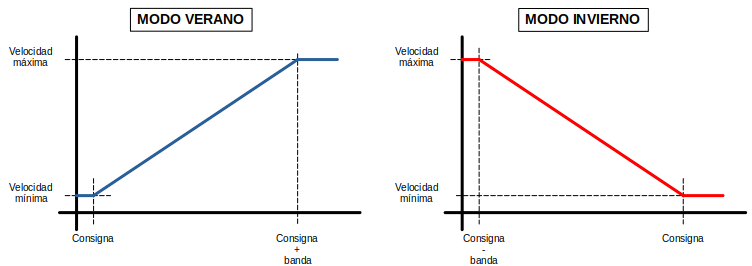
\includegraphics[width=\textwidth, keepaspectratio]{img/curvaModos}
  \caption{Modos de funcionamiento}
  \label{figura:curvasModos}
\end{figure}

%%
\begin{figure}[H]
  \centering
  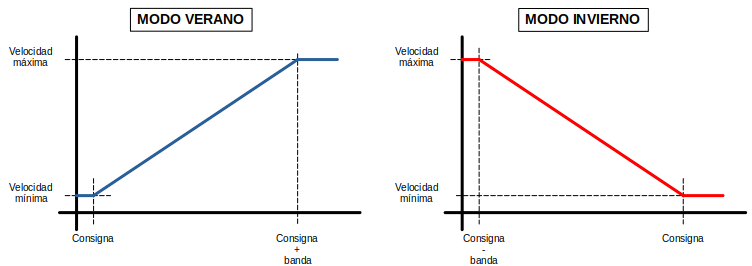
\includegraphics[width=\textwidth, keepaspectratio]{img/curvaModos}
  \caption{Modos de funcionamientoxxx}
  \label{figura:curvasModos}
\end{figure}

El \hyperref[chap:anexoProgramaUTA]{Anexo~\ref{chap:anexoProgramaUTA}} recoge el parte del programa realizado para el funcionamiento de la UTA. Los parámetros necesarios para la configuración del controlador son los de la \hyperref[chap:anexoProgramaUTA]{Tabla~\ref{chap:anexoProgramaUTA}xxx}

% Tabla xxx

\section{Diseño Pantalla para el control}
\label{sec:programacionpantalla}
Desde el programa Visoprog, donde se diseña la pantalla, se importan las variables del programa creado con el software ISaGRAF. Para ello, Visoprog tiene dos opciones de importación: directamente desde un proyecto ISaGRAF o desde una hoja excel o fichero csv. El diseño generado y el funcionamiento de la pantalla es el siguiente:

% Funcionamiento pantalla xxx según manual

\section{Elaboración de librerías en Kiconex}
\label{sec:librerias}
En el capítulo anterior se explicaba que son necesarias librerias que recopilen los registros de cada control para la integración del mismo en la plataforma IoT de kiconex. Los controles que componen la instalación del supermercado son los siguientes:

\begin{itemize}
  \item \textbf{Dixell XW60VS}: para cámaras frigoríficas y obradores.
  \item \textbf{Dixell XW60VS}: para murales, semimurales, vitrinas e islas de congelados.
  \item \textbf{Danfoss AK-PC-551}: para murales de lácteos.
  \item \textbf{Nuevo control basado en iPro IPG208}: el control programado en el apartado anterior, destinado a la UTA.
\end{itemize}

Para todos los controles existen ya librerías preparadas en kiconex, excepto para el iPro de la UTA, para el que hay que crearla a partir del programa realizado. 

ISaGRAF permite exportar un recopilatorio de variables en formato PDF. La mayoría de lo que aparece en dicho PDF se puede omitir en la librería por tratarse de parámetros por defecto del control, por lo que se han recopilado en el \hyperref[chap:anexoRegistrosUTA]{Tabla~\ref{chap:anexoRegistrosUTA}xxx} los registros que sí hay que tener en cuenta. Para añadir dichos registros a una librería, es necesario completar los siguientes campos de la pestaña librerías en la plataforma IoT:

\begin{itemize}
  \item Nombre\footnote[1]{Campo obligatorio.}
  \item Descripción\footnotemark[1]
  \item Categoría\footnotemark[1]
  \item Grupo
  \item Unidad de medida
  \item Rango
  \item \textbf{Registro\footnotemark[1]}
  \item Función de lectura
  \item Función de escritura
  \item Offset
  \item Longitud (bits)\footnotemark[1]
  \item Máscara
  \item Valor
  \item Metadatos
\end{itemize}

La \textit{categoría} clasifica clasifica al registro en función de su naturaleza (E/S, Parámetro, Alarma, etc.), y el \textit{grupo} lo clasifica en función de la aplicación (ejemplo: ventiladores, compresores, etc.). Los campos \textit{offset}, \textit{mácara} y \textit{valor} permiten hacer un tratamiento del valor que se lee o que se va a escribir, lo que es útil en situaciones en las que, por ejemplo, solo se quiere escribir un bit concreto de un campo de 8 bits, o cuando se leen datos de temperatura con campos decimales (el valor leído necesita la aplicación de un offset que indique cuántos decimales tiene).
El campo \textit{icono} permite tener un icono asociado al valor de cara a los diagramas de la plataforma.
Los \textit{metadatos} asocian valores a un campo de texto o a un icono. Por ejemplo, el estado de un ventilador se asocia a dos iconos: uno de un ventilador apagado y otro de un ventilador encendido, lo que hace que en la ventana principal se indique el estado de dicho ventilador a través de un icono en lugar de un valor, lo que lo hace más visual. Esto se aplica también a los diagramas. 

\hspace{1em}

El aspecto de la interfaz  para introducir los campos anteriores son los de las Figuras \hyperref[figura:lib0]{\ref{figura:lib0}} a \hyperref[figura:lib4]{\ref{figura:lib4}}.

\begin{figure}[H]
  \centering
  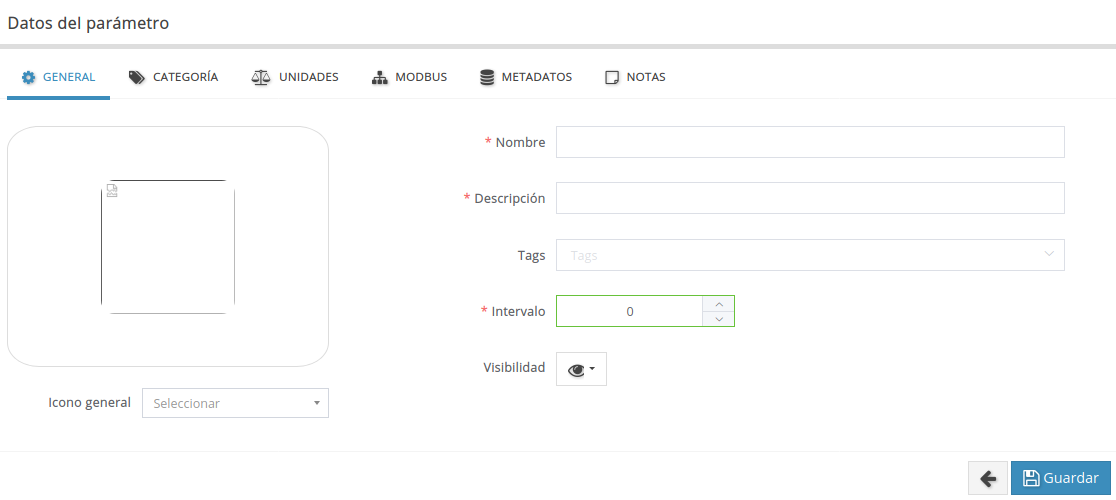
\includegraphics[width=\textwidth, keepaspectratio]{img/lib0}
  \caption{Añadir parámetro a librería kiconex - Pestaña general}
  \label{figura:lib0}
\end{figure}

\begin{figure}[H]
  \centering
  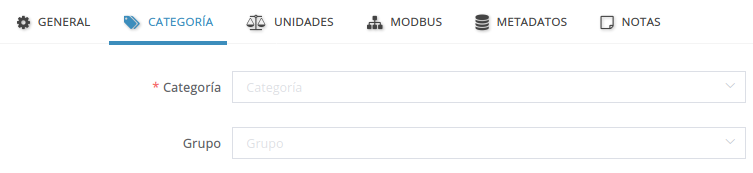
\includegraphics[width=\textwidth, keepaspectratio]{img/lib1}
  \caption{Añadir parámetro a librería kiconex - Pestaña categoría}
  \label{figura:lib1}
\end{figure}

\begin{figure}[H]
  \centering
  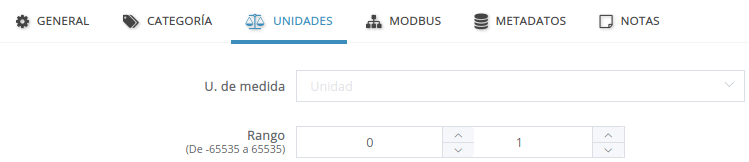
\includegraphics[width=\textwidth, keepaspectratio]{img/lib2}
  \caption{Añadir parámetro a librería kiconex - Pestaña unidades}
  \label{figura:lib2}
\end{figure}

\begin{figure}[H]
  \centering
  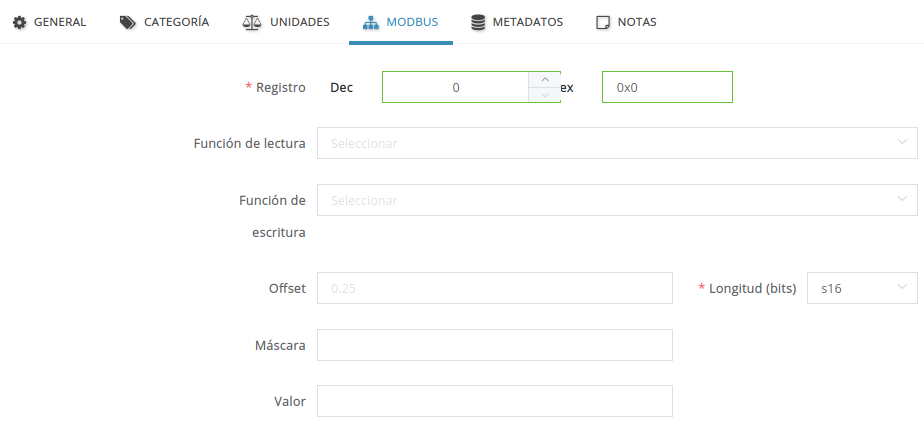
\includegraphics[width=\textwidth, keepaspectratio]{img/lib3}
  \caption{Añadir parámetro a librería kiconex - Pestaña modbus}
  \label{figura:lib3}
\end{figure}

\begin{figure}[H]
  \centering
  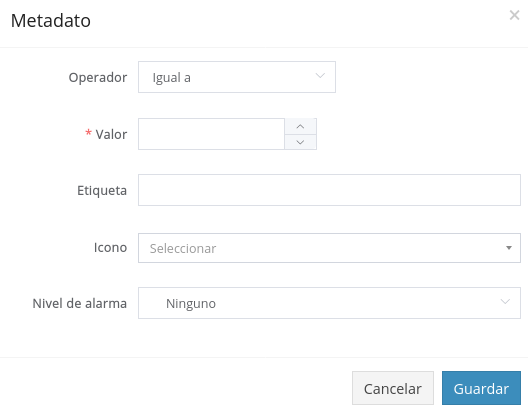
\includegraphics[width=12cm, keepaspectratio]{img/lib4}
  \caption{Añadir parámetro a librería kiconex - adición de metadato}
  \label{figura:lib4}
\end{figure}

\section{Programación dispositivo wireless}
\label{sec:programacionesp32}
Llegados a este punto, hay que buscar la forma de conectar de forma inalámbrica los muebles de refrigeración: murales de lácteos, vitrinas expositoras, semimurales e islas de congelados. Para ello se ha diseñado un nuevo dispositivo que se conecta de forma cableada al control del equipo y de forma inalámbrica a través de una red WiFi. Ya se describió en el capítulo anterior el hardware a emplear, el ESP32-PoE de Olimex, y se explicó el funcionamiento de una red kiconex. Es por ello que el software del ESP32 debe tener una serie de requisitos:

\begin{itemize}
  \item Comunicación: debe disponer de una interfaz de configuración de red, tanto de la red Modbus como de la red TCP/IP.
  \item Esclavo Modbus TCP: debe ser capaz de recibir las tramas Modbus TCP del maestro kibox, entenderlas y procesarlas para extraer cada campo.
  \item Maestro Modbus RTU: a través de la información extraída de la trama TCP recibida, enviar una nueva trama a través de Modbus RTU.
  \item Respuesta: es necesario repetir el proceso a la inversa: recibir la respuesta a la trama enviada por Modbus RTU, extraer la información y reenviarla como respuesta a la trama Modbus TCP recibida previamente desde el Maestro kibox.
\end{itemize}

\subsection{Librería para interfaz de configuración}
\label{subsec:interfazKiwi}
Para la interfaz se parte de la librería WiFiManager de Khoi Hoang~\cite{libreriaWiFigithub} \href{https://github.com/khoih-prog/ESP_WiFiManager}{(consultar su enlace en la bibliografía para más información)}. Dicha librería ha sido configurada por completo para adaptarla a las necesidades de diseño del kiwi:

\begin{enumerate}
  \item Interfaz en cualquier modo: accesible tanto en modo AP (para realizar la configuración), como en modo cliente WiFi (para ver y cambiar la configuración realizada).
  \item Medio de conexión: permite seleccionar Ethernet o WiFi.
  \item Diseño: logo de kiwi y colores de kiconex.
  \item Nuevas ventanas con más opciones, como se muestra en la \hyperref[figura:lib5]{Figura~\ref{figura:lib4}}:

  \begin{figure}[H]
    \centering
    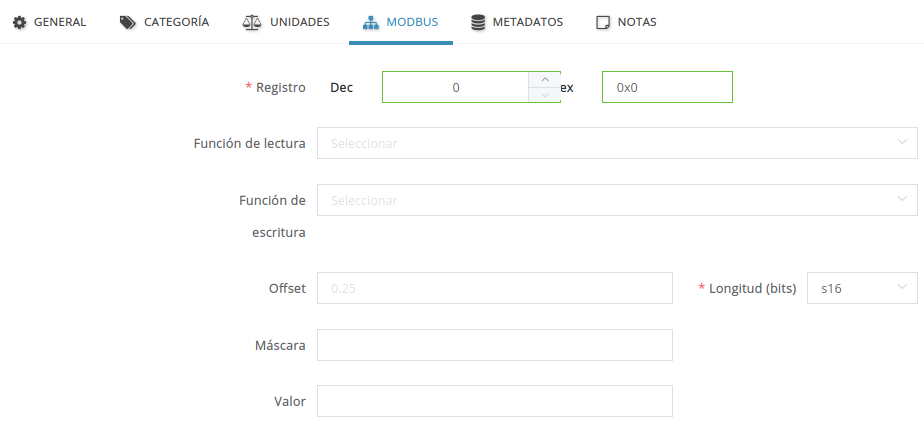
\includegraphics[width=\textwidth, keepaspectratio]{img/lib3}
    \caption{Ventanas interfaz kiwi}
    \label{figura:lib5}
  \end{figure}
\end{enumerate}

La nueva librería resultado de aplicar los anteriores cambios se ha bautizado con el nombre de KiWiManager. Su uso dentro del código principal es el siguiente:

\begin{itemize}
  \item Configuración inicial:

\begin{lstlisting}
#include <stdio.h>
#include <stdlib.h>
// programa muy positivo

void main{
  system("clear");
  printf("Hola mundo!\n");
}
\end{lstlisting}

\item Acceso al modo AP:

\begin{lstlisting}
  #include <stdio.h>
  #include <stdlib.h>
  // programa muy positivo
  
  void main{
    system("clear");
    printf("Hola mundo!\n");
  }
  \end{lstlisting}
  
  \item Conexión en modo cliente WiFi:
  
  \begin{lstlisting}
    #include <stdio.h>
    #include <stdlib.h>
    // programa muy positivo
    
    void main{
      system("clear");
      printf("Hola mundo!\n");
    }
    \end{lstlisting}
    
    \item Conexión en modo cliente Ethernet:
  
    \begin{lstlisting}
      #include <stdio.h>
      #include <stdlib.h>
      // programa muy positivo
      
      void main{
        system("clear");
        printf("Hola mundo!\n");
      }
      \end{lstlisting}  

\end{itemize}

\subsection{Librería para maestro Modbus RTU}
\label{subsec:maestroRTUkiwi}

Para esto se ha empleado la librería Modbus RTU del usuario smarmengol (Samuel Marco) en github. Para usarla dentro del código y poder enviar mensajes Modbus y recibir las respuestas, se emplea el siguiente código:

\begin{lstlisting}
  #include <stdio.h>
  #include <stdlib.h>
  // programa muy positivo
  
  void main{
    system("clear");
    printf("Hola mundo!\n");
  }
\end{lstlisting}

\subsection{Librería para esclavo Modbus TCP}
\label{subsec:esclavoTCPkiwi}

En este caso se ha diseñado por completo una librería cuya función es esperar la recepción de mensajes a través de TCP/IP a la IP del dispositivo, procesar esos mensajes y enviarlos vía Modbus RTU empleando la librería anterior. Es decir se trata de una librería puente, por lo que se ha bautizado con el nombre de KiWiModbusBridge. Su uso dentro del código principal es el siguiente:

\begin{lstlisting}
  #include <stdio.h>
  #include <stdlib.h>
  // programa muy positivo
  
  void main{
    system("clear");
    printf("Hola mundo!\n");
  }
\end{lstlisting}

En el \hyperref[chap:anexoLibreriaBridge]{Anexo~\ref{chap:anexoLibreriaBridge}} se describe la lógica de funcionamiento de esta librería.

\subsection{Código principal}
\label{subsec:mainCodeKiwi}

El código principal del software de kiwi se encarga de integrar cada una de las librerías anteriores y de gestionar el flujo de programa. Su lógica de funcionamiento se recoge en el siguiente diagrama:

\begin{figure}[H]
  \centering
  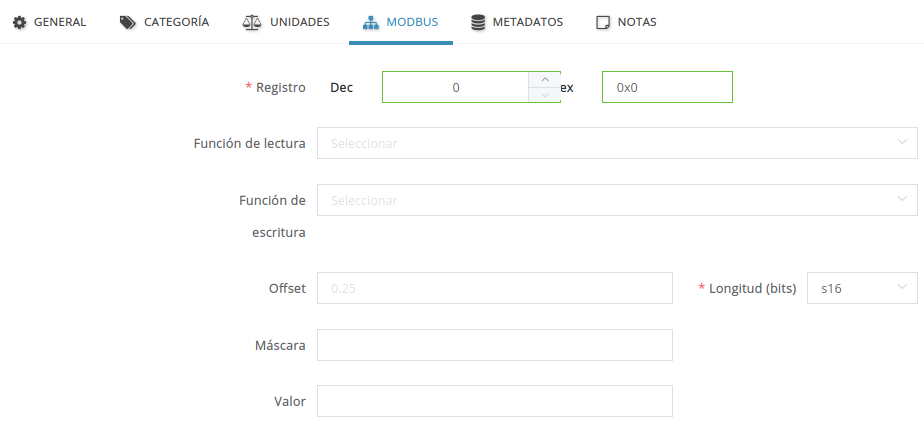
\includegraphics[width=\textwidth, keepaspectratio]{img/lib3}
  \caption{Flujo de programa del código principal de kiwi}
  \label{figura:lib6}
\end{figure}